\documentclass{ximera}

%\usepackage{todonotes}

\newcommand{\todo}{}

\usepackage{esint} % for \oiint
\ifxake%%https://math.meta.stackexchange.com/questions/9973/how-do-you-render-a-closed-surface-double-integral
\renewcommand{\oiint}{{\large\bigcirc}\kern-1.56em\iint}
\fi


\graphicspath{
  {./}
  {ximeraTutorial/}
  {basicPhilosophy/}
  {functionsOfSeveralVariables/}
  {normalVectors/}
  {lagrangeMultipliers/}
  {vectorFields/}
  {greensTheorem/}
  {shapeOfThingsToCome/}
  {dotProducts/}
  {partialDerivativesAndTheGradientVector/}
  {../productAndQuotientRules/exercises/}
  {../normalVectors/exercisesParametricPlots/}
  {../continuityOfFunctionsOfSeveralVariables/exercises/}
  {../partialDerivativesAndTheGradientVector/exercises/}
  {../directionalDerivativeAndChainRule/exercises/}
  {../commonCoordinates/exercisesCylindricalCoordinates/}
  {../commonCoordinates/exercisesSphericalCoordinates/}
  {../greensTheorem/exercisesCurlAndLineIntegrals/}
  {../greensTheorem/exercisesDivergenceAndLineIntegrals/}
  {../shapeOfThingsToCome/exercisesDivergenceTheorem/}
  {../greensTheorem/}
  {../shapeOfThingsToCome/}
  {../separableDifferentialEquations/exercises/}
  {vectorFields/}
}

\newcommand{\mooculus}{\textsf{\textbf{MOOC}\textnormal{\textsf{ULUS}}}}

\usepackage{tkz-euclide}
\usepackage{tikz}
\usepackage{tikz-cd}
\usetikzlibrary{arrows}
\tikzset{>=stealth,commutative diagrams/.cd,
  arrow style=tikz,diagrams={>=stealth}} %% cool arrow head
\tikzset{shorten <>/.style={ shorten >=#1, shorten <=#1 } } %% allows shorter vectors

\usetikzlibrary{backgrounds} %% for boxes around graphs
\usetikzlibrary{shapes,positioning}  %% Clouds and stars
\usetikzlibrary{matrix} %% for matrix
\usepgfplotslibrary{polar} %% for polar plots
\usepgfplotslibrary{fillbetween} %% to shade area between curves in TikZ
%\usetkzobj{all}
\usepackage[makeroom]{cancel} %% for strike outs
%\usepackage{mathtools} %% for pretty underbrace % Breaks Ximera
%\usepackage{multicol}
\usepackage{pgffor} %% required for integral for loops



%% http://tex.stackexchange.com/questions/66490/drawing-a-tikz-arc-specifying-the-center
%% Draws beach ball
\tikzset{pics/carc/.style args={#1:#2:#3}{code={\draw[pic actions] (#1:#3) arc(#1:#2:#3);}}}



\usepackage{array}
\setlength{\extrarowheight}{+.1cm}
\newdimen\digitwidth
\settowidth\digitwidth{9}
\def\divrule#1#2{
\noalign{\moveright#1\digitwidth
\vbox{\hrule width#2\digitwidth}}}




% \newcommand{\RR}{\mathbb R}
% \newcommand{\R}{\mathbb R}
% \newcommand{\N}{\mathbb N}
% \newcommand{\Z}{\mathbb Z}

\newcommand{\sagemath}{\textsf{SageMath}}


%\renewcommand{\d}{\,d\!}
%\renewcommand{\d}{\mathop{}\!d}
%\newcommand{\dd}[2][]{\frac{\d #1}{\d #2}}
%\newcommand{\pp}[2][]{\frac{\partial #1}{\partial #2}}
% \renewcommand{\l}{\ell}
%\newcommand{\ddx}{\frac{d}{\d x}}

% \newcommand{\zeroOverZero}{\ensuremath{\boldsymbol{\tfrac{0}{0}}}}
%\newcommand{\inftyOverInfty}{\ensuremath{\boldsymbol{\tfrac{\infty}{\infty}}}}
%\newcommand{\zeroOverInfty}{\ensuremath{\boldsymbol{\tfrac{0}{\infty}}}}
%\newcommand{\zeroTimesInfty}{\ensuremath{\small\boldsymbol{0\cdot \infty}}}
%\newcommand{\inftyMinusInfty}{\ensuremath{\small\boldsymbol{\infty - \infty}}}
%\newcommand{\oneToInfty}{\ensuremath{\boldsymbol{1^\infty}}}
%\newcommand{\zeroToZero}{\ensuremath{\boldsymbol{0^0}}}
%\newcommand{\inftyToZero}{\ensuremath{\boldsymbol{\infty^0}}}



% \newcommand{\numOverZero}{\ensuremath{\boldsymbol{\tfrac{\#}{0}}}}
% \newcommand{\dfn}{\textbf}
% \newcommand{\unit}{\,\mathrm}
% \newcommand{\unit}{\mathop{}\!\mathrm}
% \newcommand{\eval}[1]{\bigg[ #1 \bigg]}
% \newcommand{\seq}[1]{\left( #1 \right)}
% \renewcommand{\epsilon}{\varepsilon}
% \renewcommand{\phi}{\varphi}


% \renewcommand{\iff}{\Leftrightarrow}

% \DeclareMathOperator{\arccot}{arccot}
% \DeclareMathOperator{\arcsec}{arcsec}
% \DeclareMathOperator{\arccsc}{arccsc}
% \DeclareMathOperator{\si}{Si}
% \DeclareMathOperator{\scal}{scal}
% \DeclareMathOperator{\sign}{sign}


%% \newcommand{\tightoverset}[2]{% for arrow vec
%%   \mathop{#2}\limits^{\vbox to -.5ex{\kern-0.75ex\hbox{$#1$}\vss}}}
% \newcommand{\arrowvec}[1]{{\overset{\rightharpoonup}{#1}}}
% \renewcommand{\vec}[1]{\arrowvec{\mathbf{#1}}}
% \renewcommand{\vec}[1]{{\overset{\boldsymbol{\rightharpoonup}}{\mathbf{#1}}}}

% \newcommand{\point}[1]{\left(#1\right)} %this allows \vector{ to be changed to \vector{ with a quick find and replace
% \newcommand{\pt}[1]{\mathbf{#1}} %this allows \vec{ to be changed to \vec{ with a quick find and replace
% \newcommand{\Lim}[2]{\lim_{\point{#1} \to \point{#2}}} %Bart, I changed this to point since I want to use it.  It runs through both of the exercise and exerciseE files in limits section, which is why it was in each document to start with.

% \DeclareMathOperator{\proj}{\mathbf{proj}}
% \newcommand{\veci}{{\boldsymbol{\hat{\imath}}}}
% \newcommand{\vecj}{{\boldsymbol{\hat{\jmath}}}}
% \newcommand{\veck}{{\boldsymbol{\hat{k}}}}
% \newcommand{\vecl}{\vec{\boldsymbol{\l}}}
% \newcommand{\uvec}[1]{\mathbf{\hat{#1}}}
% \newcommand{\utan}{\mathbf{\hat{t}}}
% \newcommand{\unormal}{\mathbf{\hat{n}}}
% \newcommand{\ubinormal}{\mathbf{\hat{b}}}

% \newcommand{\dotp}{\bullet}
% \newcommand{\cross}{\boldsymbol\times}
% \newcommand{\grad}{\boldsymbol\nabla}
% \newcommand{\divergence}{\grad\dotp}
% \newcommand{\curl}{\grad\cross}
%\DeclareMathOperator{\divergence}{divergence}
%\DeclareMathOperator{\curl}[1]{\grad\cross #1}
% \newcommand{\lto}{\mathop{\longrightarrow\,}\limits}

% \renewcommand{\bar}{\overline}

\colorlet{textColor}{black}
\colorlet{background}{white}
\colorlet{penColor}{blue!50!black} % Color of a curve in a plot
\colorlet{penColor2}{red!50!black}% Color of a curve in a plot
\colorlet{penColor3}{red!50!blue} % Color of a curve in a plot
\colorlet{penColor4}{green!50!black} % Color of a curve in a plot
\colorlet{penColor5}{orange!80!black} % Color of a curve in a plot
\colorlet{penColor6}{yellow!70!black} % Color of a curve in a plot
\colorlet{fill1}{penColor!20} % Color of fill in a plot
\colorlet{fill2}{penColor2!20} % Color of fill in a plot
\colorlet{fillp}{fill1} % Color of positive area
\colorlet{filln}{penColor2!20} % Color of negative area
\colorlet{fill3}{penColor3!20} % Fill
\colorlet{fill4}{penColor4!20} % Fill
\colorlet{fill5}{penColor5!20} % Fill
\colorlet{gridColor}{gray!50} % Color of grid in a plot

\newcommand{\surfaceColor}{violet}
\newcommand{\surfaceColorTwo}{redyellow}
\newcommand{\sliceColor}{greenyellow}




\pgfmathdeclarefunction{gauss}{2}{% gives gaussian
  \pgfmathparse{1/(#2*sqrt(2*pi))*exp(-((x-#1)^2)/(2*#2^2))}%
}


%%%%%%%%%%%%%
%% Vectors
%%%%%%%%%%%%%

%% Simple horiz vectors
\renewcommand{\vector}[1]{\left\langle #1\right\rangle}


%% %% Complex Horiz Vectors with angle brackets
%% \makeatletter
%% \renewcommand{\vector}[2][ , ]{\left\langle%
%%   \def\nextitem{\def\nextitem{#1}}%
%%   \@for \el:=#2\do{\nextitem\el}\right\rangle%
%% }
%% \makeatother

%% %% Vertical Vectors
%% \def\vector#1{\begin{bmatrix}\vecListA#1,,\end{bmatrix}}
%% \def\vecListA#1,{\if,#1,\else #1\cr \expandafter \vecListA \fi}

%%%%%%%%%%%%%
%% End of vectors
%%%%%%%%%%%%%

%\newcommand{\fullwidth}{}
%\newcommand{\normalwidth}{}



%% makes a snazzy t-chart for evaluating functions
%\newenvironment{tchart}{\rowcolors{2}{}{background!90!textColor}\array}{\endarray}

%%This is to help with formatting on future title pages.
\newenvironment{sectionOutcomes}{}{}



%% Flowchart stuff
%\tikzstyle{startstop} = [rectangle, rounded corners, minimum width=3cm, minimum height=1cm,text centered, draw=black]
%\tikzstyle{question} = [rectangle, minimum width=3cm, minimum height=1cm, text centered, draw=black]
%\tikzstyle{decision} = [trapezium, trapezium left angle=70, trapezium right angle=110, minimum width=3cm, minimum height=1cm, text centered, draw=black]
%\tikzstyle{question} = [rectangle, rounded corners, minimum width=3cm, minimum height=1cm,text centered, draw=black]
%\tikzstyle{process} = [rectangle, minimum width=3cm, minimum height=1cm, text centered, draw=black]
%\tikzstyle{decision} = [trapezium, trapezium left angle=70, trapezium right angle=110, minimum width=3cm, minimum height=1cm, text centered, draw=black]


\title{Polar Form}

\begin{document}

\begin{abstract}
locating numbers
\end{abstract}
\maketitle



\section*{Representing Complex Numbers}

We already have several ways of representing complex numbers. \\



\textbf{\textcolor{red!80!black}{$\blacktriangleright (4, 8)$}}: We represent complex numbers visually with points or dots on the Cartesian plane.  \\





\begin{image}
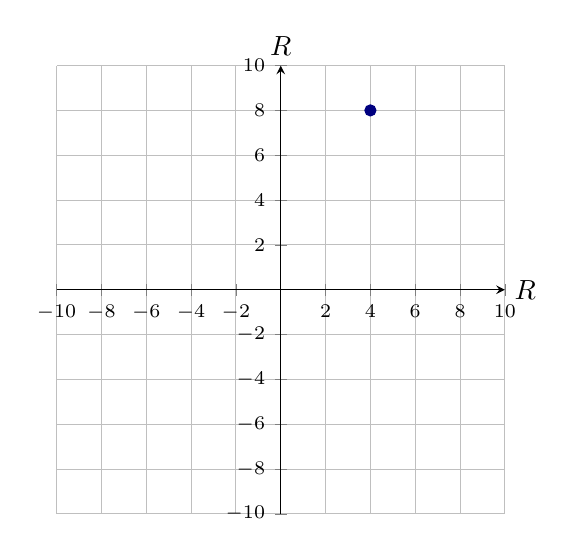
\begin{tikzpicture}
  \begin{axis}[
            domain=-10:10, ymax=10, xmax=10, ymin=-10, xmin=-10,
            axis lines =center, xlabel=$\mathbb{R}$, ylabel=$\mathbb{R}$, grid = major,
            unit vector ratio*=1 1 1,
            ytick={-10,-8,-6,-4,-2,2,4,6,8,10},
            xtick={-10,-8,-6,-4,-2,2,4,6,8,10},
            ticklabel style={font=\scriptsize},
            every axis y label/.style={at=(current axis.above origin),anchor=south},
            every axis x label/.style={at=(current axis.right of origin),anchor=west},
            axis on top
          ]
          

          \addplot[color=penColor,fill=penColor,only marks,mark=*] coordinates{(4,8)};



  \end{axis}
\end{tikzpicture}
\end{image}








\textbf{\textcolor{red!80!black}{$\blacktriangleright \langle 4, 8 \rangle$}}: We represent complex numbers with vectors.  These are illustrated with arrows on the Cartesian plane.  Algebraically, we write vectors using triangular brackets.






\begin{image}
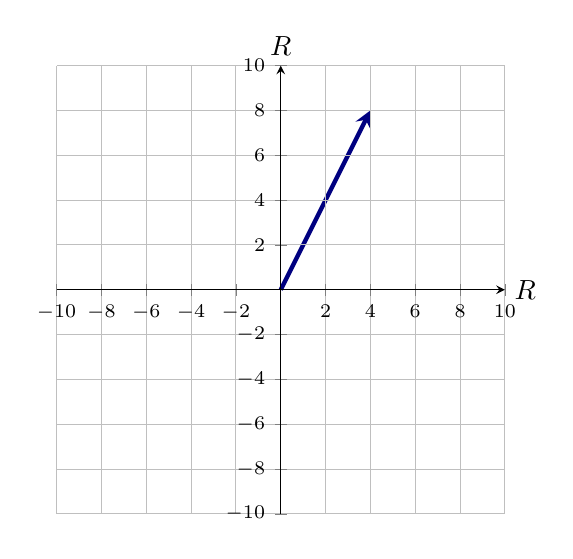
\begin{tikzpicture}
  \begin{axis}[
            domain=-10:10, ymax=10, xmax=10, ymin=-10, xmin=-10,
            axis lines =center, xlabel=$\mathbb{R}$, ylabel=$\mathbb{R}$, grid = major,
            unit vector ratio*=1 1 1,
            ytick={-10,-8,-6,-4,-2,2,4,6,8,10},
            xtick={-10,-8,-6,-4,-2,2,4,6,8,10},
            ticklabel style={font=\scriptsize},
            every axis y label/.style={at=(current axis.above origin),anchor=south},
            every axis x label/.style={at=(current axis.right of origin),anchor=west},
            axis on top
          ]
          

          \draw[penColor,ultra thick,->] (axis cs:0,0) -- (axis cs:4,8);


  \end{axis}
\end{tikzpicture}
\end{image}

Vectors have a visual arithmetic, where we arrange the vectors tail-to-head or tail-to-tail and then create a resultant vector from the arrangement. These resultant vectors represent the sum or difference of two Complex numbers.

Vectors have a symbolic arithmetic as well, which agrees with the geometric operations:

\[
\langle a, b \rangle + \langle c, d \rangle = \langle a+c, b+d \rangle
\]



\textbf{\textcolor{red!90!darkgray}{$\blacktriangleright 4 + 8 \, i$}}: We represent complex numbers with a 2-dimensional sum.



The left, first, or horizontal part is called the \textbf{\textcolor{purple!85!blue}{real part}} and the right, second, or vertical part is called the \textbf{\textcolor{purple!85!blue}{imaginary part}}.



When viewing the plane in this context, we call it the \textbf{\textcolor{purple!85!blue}{Complex Plane}}.





\begin{image}
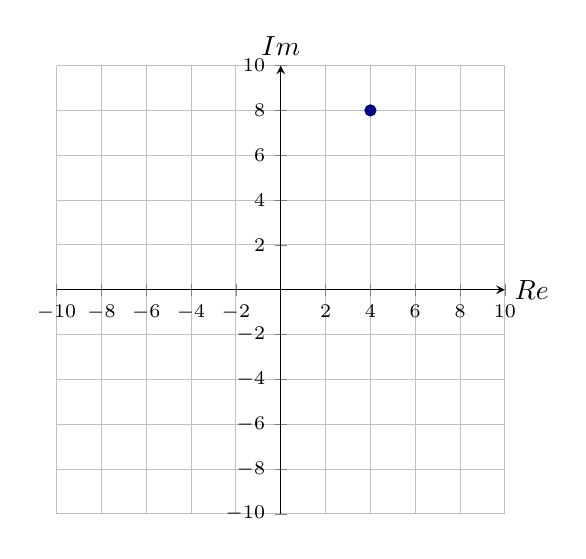
\begin{tikzpicture}
  \begin{axis}[
            domain=-10:10, ymax=10, xmax=10, ymin=-10, xmin=-10,
            axis lines =center, xlabel=$Re$, ylabel=$Im$, grid = major,
            unit vector ratio*=1 1 1,
            ytick={-10,-8,-6,-4,-2,2,4,6,8,10},
            xtick={-10,-8,-6,-4,-2,2,4,6,8,10},
            ticklabel style={font=\scriptsize},
            every axis y label/.style={at=(current axis.above origin),anchor=south},
            every axis x label/.style={at=(current axis.right of origin),anchor=west},
            axis on top
          ]
          

          \addplot[color=penColor,fill=penColor,only marks,mark=*] coordinates{(4,8)};


  \end{axis}
\end{tikzpicture}
\end{image}






All of these representations share a common structure.  They all describe complex numbers with rectangular measurements.  All of the descriptions above give horizontal (left/right) and vertical (up/down) information.


There is a different way to describe complex numbers.






\begin{warning} \textbf{\textcolor{red!80!black}{Context}}


Mathematics is famous for reusing notation.  We use the exact same symbols to represent different mathematical objects and we let the context of the situation dictate our interpretation. \\

Same story here. \\

Just like with Real Numbers, we have geometric and algebraic representations of Complex Numbers.  The geometric representations and symbols are borrowed from our Geometry.


$(a, b)$ might represent an interval in the real numbers.  It might represent the coordinates of a point in the Cartesian plane.  It might represent a Complex number. \\

$\langle a, b \rangle$ might represent a vector.  It might represent an arrow in the Cartesian plane.  It might represent a Complex number. \\

This is normal. It happens every day with the English langugae.  We need to take into account the people and context of the discussion.
\end{warning}












\section*{Polar Coordinates}

Instead of rectangular information, we could give circular information.  We could give the angle the vector makes with the positive horizontal axis together with the length or distance from the origin. 

In keeping with the circular idea, the vector resembles a radius.  

Our two pieces of information will be $r$ and $\theta$. These are known as \textbf{polar coordinates}




\begin{definition}   \textbf{\textcolor{green!50!black}{Polar Coordinates}} \\

Each Complex number can be described by $(r, \theta)$, where $r$ is a real number and $\theta$ is an angle measurement.  \\


$r$ can be positive or negative. \\
$\theta$ is measured counterclockwise from the positive real axis. \\

\end{definition}


Of course, that is how we write rectangular coordinates as well.  The context of the situation will tell us how to interpret the coordinates.



\begin{example}



Write $4 + 8i$ in polar form.



\begin{image}
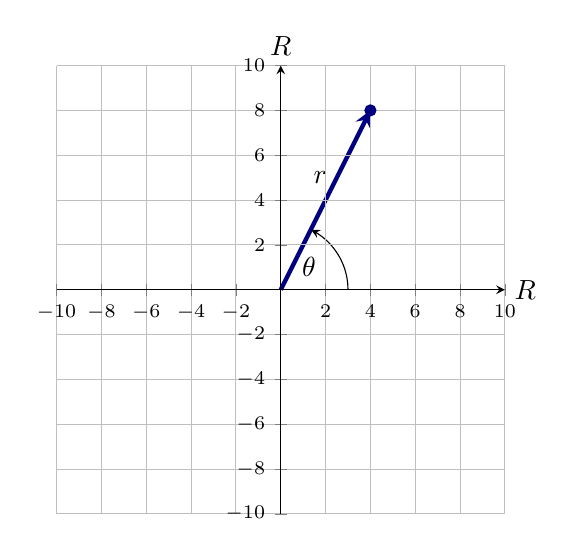
\begin{tikzpicture}
  \begin{axis}[
            domain=-10:10, ymax=10, xmax=10, ymin=-10, xmin=-10,
            axis lines =center, xlabel=$\mathbb{R}$, ylabel=$\mathbb{R}$, grid = major,
            unit vector ratio*=1 1 1,
            ytick={-10,-8,-6,-4,-2,2,4,6,8,10},
            xtick={-10,-8,-6,-4,-2,2,4,6,8,10},
            ticklabel style={font=\scriptsize},
            every axis y label/.style={at=(current axis.above origin),anchor=south},
            every axis x label/.style={at=(current axis.right of origin),anchor=west},
            axis on top
          ]
          
          \addplot[color=penColor,fill=penColor,only marks,mark=*] coordinates{(4,8)};
          \draw[penColor,ultra thick,->] (axis cs:0,0) -- (axis cs:4,8);
          \addplot [textColor,smooth, domain=(0:63),->] ({3*cos(x)},{3*sin(x)});
          \node at (axis cs:2,1) [anchor=east] {$\theta$};
          \node at (axis cs:2.5,5) [anchor=east] {$r$};


           

  \end{axis}
\end{tikzpicture}
\end{image}


$r = \sqrt{4^2 + 8^2} = \sqrt{80} = 4\sqrt{5}$ (the modulus of $4 + 8 \, i$) \\
We need $\theta$ to give us $\tan(\theta) = 2$, which is approximately $\theta \approx 63.43^{\circ}$ \\



We, again, wrap the coordinates up with parentheses: $(r, \theta) = (16\sqrt{5}, 63.43^{\circ})$.


And, we need to work equally well with radians and degrees: $(r, \theta) = (16\sqrt{5}, 1.107)$


\end{example}












\begin{warning} \textbf{\textcolor{red!80!black}{Multiple Polar Coordinates}}


Unlike with rectangular coordinates, different polar coordinates can describe the same complex number.

\[
 \cdots = (r, \theta - 2\pi) = (r, \theta) = (r, \theta + 2\pi) = (r, \theta + 4\pi) = \cdots
\]

\end{warning}






\begin{warning} \textbf{\textcolor{red!80!black}{Negative ``Distance''}}


The $r$ in $(r, \theta)$ is the distance to move in the $\theta$-direction.  However, $r$ can be negative. In this case, the interpretation is to move in the opposite direction from $\theta$.

\[
 (r, \theta) = (-r, \theta + \pi) = (-r, \theta - \pi)
\]

\end{warning}








  \begin{image}
    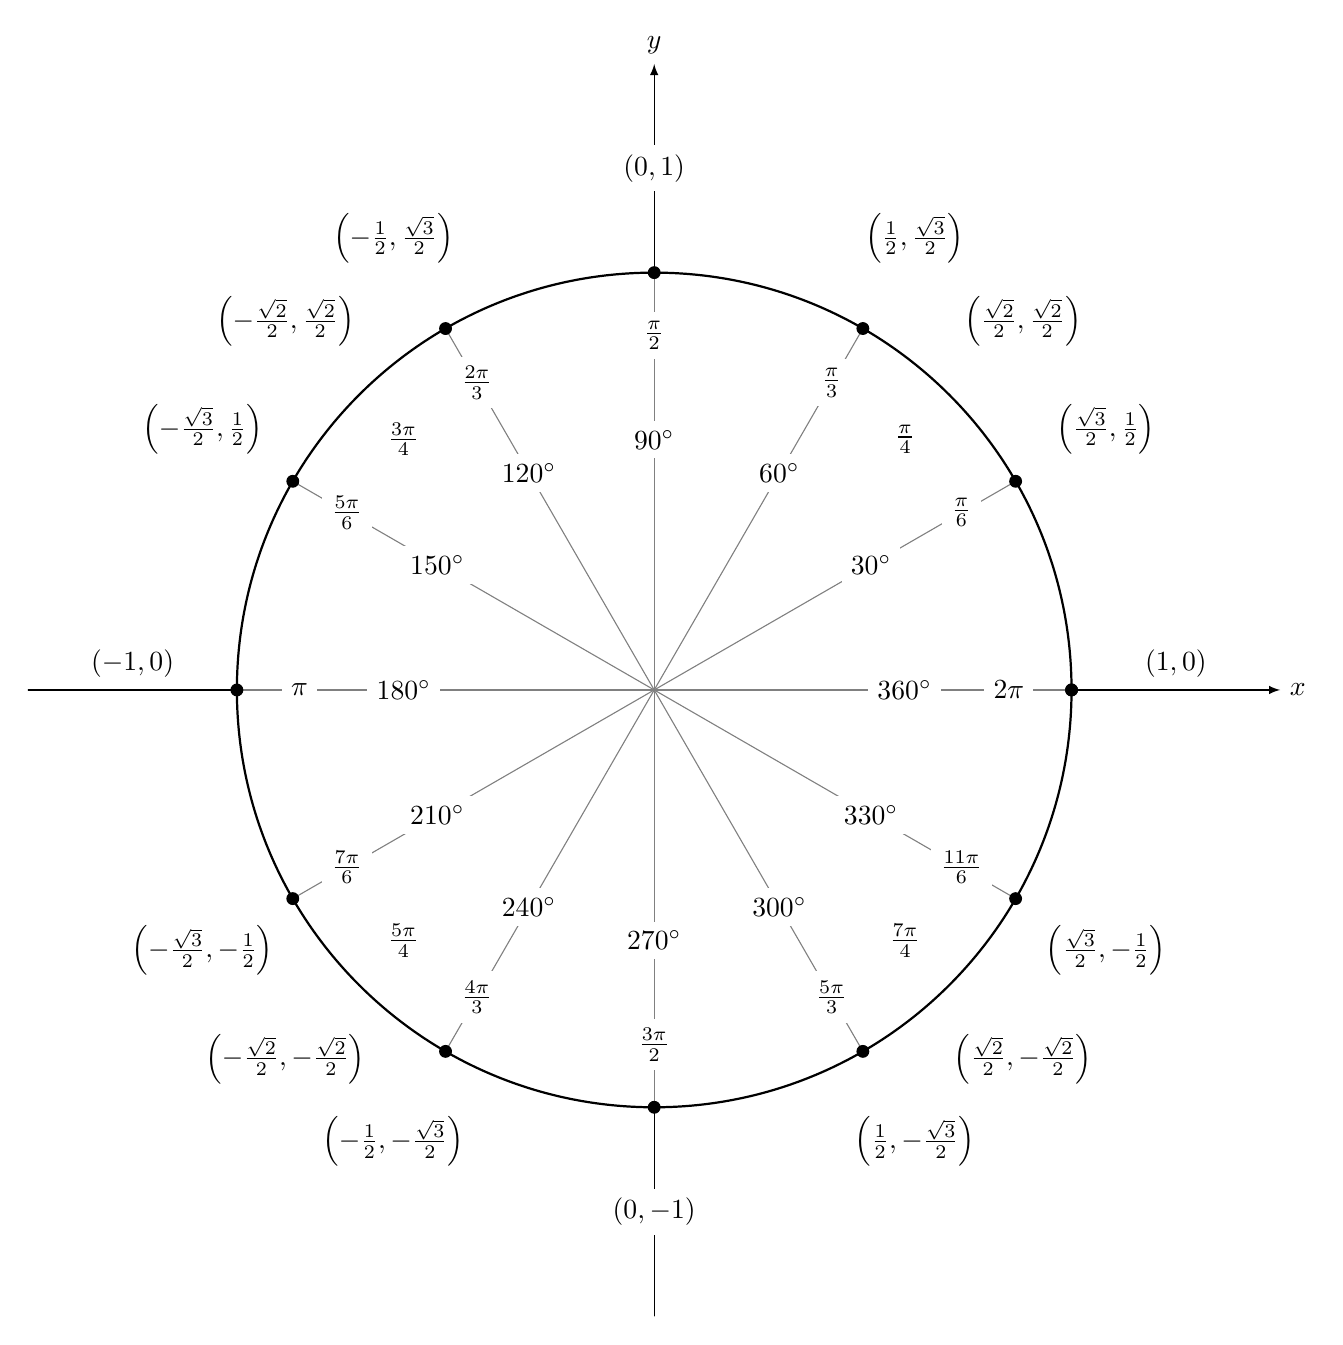
\begin{tikzpicture}[scale=5.3,cap=round,>=latex]
        % draw the coordinates
        \draw[->] (-1.5cm,0cm) -- (1.5cm,0cm) node[right,fill=white] {$x$};
        \draw[->] (0cm,-1.5cm) -- (0cm,1.5cm) node[above,fill=white] {$y$};

        % draw the unit circle
        \draw[thick] (0cm,0cm) circle(1cm);

        \foreach \x in {0,30,...,360} {
                % lines from center to point
                \draw[gray] (0cm,0cm) -- (\x:1cm);
                % dots at each point
                \filldraw[black] (\x:1cm) circle(0.4pt);
                % draw each angle in degrees
                \draw (\x:0.6cm) node[fill=white] {$\x^\circ$};
        }

        % draw each angle in radians
        \foreach \x/\xtext in {
            30/\frac{\pi}{6},
            45/\frac{\pi}{4},
            60/\frac{\pi}{3},
            90/\frac{\pi}{2},
            120/\frac{2\pi}{3},
            135/\frac{3\pi}{4},
            150/\frac{5\pi}{6},
            180/\pi,
            210/\frac{7\pi}{6},
            225/\frac{5\pi}{4},
            240/\frac{4\pi}{3},
            270/\frac{3\pi}{2},
            300/\frac{5\pi}{3},
            315/\frac{7\pi}{4},
            330/\frac{11\pi}{6},
            360/2\pi}
                \draw (\x:0.85cm) node[fill=white] {$\xtext$};

        \foreach \x/\xtext/\y in {
            % the coordinates for the first quadrant
            30/\frac{\sqrt{3}}{2}/\frac{1}{2},
            45/\frac{\sqrt{2}}{2}/\frac{\sqrt{2}}{2},
            60/\frac{1}{2}/\frac{\sqrt{3}}{2},
            % the coordinates for the second quadrant
            150/-\frac{\sqrt{3}}{2}/\frac{1}{2},
            135/-\frac{\sqrt{2}}{2}/\frac{\sqrt{2}}{2},
            120/-\frac{1}{2}/\frac{\sqrt{3}}{2},
            % the coordinates for the third quadrant
            210/-\frac{\sqrt{3}}{2}/-\frac{1}{2},
            225/-\frac{\sqrt{2}}{2}/-\frac{\sqrt{2}}{2},
            240/-\frac{1}{2}/-\frac{\sqrt{3}}{2},
            % the coordinates for the fourth quadrant
            330/\frac{\sqrt{3}}{2}/-\frac{1}{2},
            315/\frac{\sqrt{2}}{2}/-\frac{\sqrt{2}}{2},
            300/\frac{1}{2}/-\frac{\sqrt{3}}{2}}
                \draw (\x:1.25cm) node[fill=white] {$\left(\xtext,\y\right)$};

        % draw the horizontal and vertical coordinates
        % the placement is better this way
        \draw (-1.25cm,0cm) node[above=1pt] {$(-1,0)$}
              (1.25cm,0cm)  node[above=1pt] {$(1,0)$}
              (0cm,-1.25cm) node[fill=white] {$(0,-1)$}
              (0cm,1.25cm)  node[fill=white] {$(0,1)$};
    \end{tikzpicture}
  \end{image}








\begin{question}
Which of the following polar coordinates represent the same complex number?
\begin{selectAll}
\choice[correct]{$\left( 5, \frac{\pi}{4} \right)$}
\choice[correct]{$\left( 5, \frac{9\pi}{4} \right)$}
\choice{$\left( 5, \frac{3\pi}{4} \right)$}
\choice[correct]{$\left( -5, \frac{5\pi}{4} \right)$}
\choice{$\left( -5, \frac{7\pi}{4} \right)$}
\end{selectAll}
\end{question}








\begin{warning} \textbf{\textcolor{red!80!black}{Radians}}


There is a very tight relationship between angles and arc length in the unit circle. \\


A full unit circle is $2\pi$ radians and the circumference is $2\pi$. When measuring in radians, the angle is the same value as the arc length.  As you rotate around the unit circle that angles changes at exactly the same rate as the arc length. \\

This relationship does not hold with degrees. A full unit circle is $360$ degrees, which is not matching  the circumference at $2\pi$. \\


For this reason, Calculus uses radians almost exclusively.  In Precalculus, we need to become radian thinkers.





\end{warning}









\begin{center}
\textbf{\textcolor{green!50!black}{oooooo-=-=-=-ooOoo-=-=-=-ooooo}} \\

more examples can be found by following this link\\ \link[More Examples of Polar Form of Complex Numbers]{https://ximera.osu.edu/csccmathematics/precalculus2/precalculus2/polarFormComplexNumbers/examples/exampleList}

\end{center}


\end{document}
